%% ----------------------------------------------------------------
%% Project.tex
%% ---------------------------------------------------------------- 
\documentclass{ecsreport}     				% Use the Project Style
\graphicspath{{../Figures-Interim/}}   		% Location of your graphics files
\usepackage[square,numbers]{natbib}   	% Use Natbib style for the refs.
\hypersetup{colorlinks=true}   			% Set to false for black/white printing
%\begin{document}
def
\end{document}            			% Include your abbreviations
\setboolean{@twoside}{false}				% We don't want a page gutter
%% ----------------------------------------------------------------
\begin{document}
\frontmatter
\title      {Speech Recognition on Embedded Hardware}
\authors    {\texorpdfstring
             {\href{mailto:rmds1g10@ecs.soton.ac.uk}{Ricardo da Silva}}
             {Ricardo da Silva}
            }
\addresses  {\groupname\\\deptname\\\univname}
\date       {\today}
\subject    {}
\keywords   {}
\supervisor {Dr Steve Gunn}
\examiner   {Dr Nick Harris}
\degree     {MEng Electronic Engineering with Mobile and Secure Systems}
\maketitle
\begin{abstract}
This interim report discusses the progress and plans of work towards a project about speech recognition for embedded systems.  The overall goals of this project are outlined, and background information on various aspects of the project is given, along with details from various knowledge sources.  The technical progress that that has been made is discussed, followed by plans for the remaining work.
\end{abstract}
\tableofcontents
%\listoffigures
%\listoftables
%\lstlistoflistings
%\listofsymbols{ll}{$w$ & The weight vector}
%\acknowledgements{Thanks to no one.}
%\dedicatory{To \dots}
\mainmatter
%% ----------------------------------------------------------------

\section{Introduction} % (fold)
\label{sec:introduction}
Speech recognition is an interesting computational problem, for which there is no fool-proof solution at this time.  Recently the industry for embedded devices and small-scale digital systems has expanded greatly, but in general these devices do not have the power or speed to run speech recognition.  Field Programmable Gate Arrays (FPGAs) may present a way of increasing the capability of such systems, as they are able to perform calculations much faster than traditional microprocessors.
% section introduction (end)


%!TEX root = main.tex
% 243 words
\chapter{Project Goals} % (fold)
\label{cha:goals}

At the highest level, the goal of this project is to develop a speech recognition system that will run on embedded hardware.  In pursuing this goal, the aim is to achieve several other goals that will be beneficial to the author and to the University of Southampton.

\section{Speech Recognition} % (fold)
\label{sec:speech_recognition}
The speech recognition system proposed aims to be run using an ARM chip doing pre-processing and an FPGA doing statistical decoding.  Ideally, it will be capable of performing HMM based speaker-independent speech recognition.  This, however, is very ambitious, and so initially the project will focus on getting the most basic forms of the relevant algorithms running in software.  Once this is complete, the system will be built into hardware, and extended to be more complete.
% section speech_recognition (end)

\section{The Micro Arcana} % (fold)
\label{sec:the_micro_arcana}
In terms of hardware, one of the project goals is to further development of the Micro Arcana family of boards, currently under development by Dr Steve Gunn.  
The speech recognition system proposed will make use of two of the boards -- the ``L'Imperatrice'' ARM based mini-computer, and the ``La Papessa'' FPGA board.  Part of the project is setting up and configuring these two boards, and having a finished system will help demonstrate their capabilities.
% section the_micro_arcana (end)

\section{Theoretical understanding} % (fold)
\label{sec:theoretical_understanding}
A major goal of the project is to develop a higher level of understanding of the algorithms used in speech recognition, and to get experience designing a large-scale embedded application.  This complements the intrests of the author and the subjects being studied, in particular, Intelligent Algorithms and Digital Systems Design.
% section theoretical_understanding (end)


% chapter goals (end)

%!TEX root = main.tex
% 1265 words
\chapter{Background and Investigations} % (fold)
\label{cha:background}

\section{Speech Recognition Systems} % (fold)
\label{sec:speech_recognition_systems}
In general, `Speech Recognition' refers to the process of translating spoken words or phrases into a form that can be understood by an electronic system, which usually means using mathematical models and methods to process and then decode the sound signal.  Translating a speech waveform into this form typically requires three main steps \cite{melnikoff2003speech}.  The raw waveform must be converted into an `observation vector', which is a set of data that is compatible with the chosen speech model.  This data is then sent through a decoder, which attempts to recognise which words or sub-word units were spoken.  These are then sent through a language model, which imposes rules on what combinations of words of syntax are allowed.  This project aims to focus on the first and second tasks, as they are the more interesting from an electronic engineering point of view.

There are a variety of different methods and models that have been used to perform speech recognition.  An overview of the most popular will be described here, along with the chosen approach.

\subsection{Tor's Algorithm} % (fold)
\label{sub:tors_algorithm}
The author first became interested in speech recognition when reading about ``Tor's Algorithm'', which is a very simple small dictionary speech recognition system \cite{tor2003}.  This algorithm is capable of very accurate speaker dependent speech recognition for a dictionary of less than ten words.  It is based on a fingerprinting model where each word in the dictionary must be trained to form an acoustic `fingerprint'.  This fingerprint is based on the time variations of the speech signal after being filtered appropriately.  Then recognition is reduced to finding the Euclidean distance squared between the input vector and each of the stored fingerprints.  The `closest' match is the word with the smallest distance from the input.
Although this system is very simplistic, it outlines two major components of any speech recognition system -- pre-processing and decoding (recognition).  More complex systems just use more complex speech models and pre-processing methods.
% subsection tors_algorithm (end)

\subsection{Dynamic Time Warping} % (fold)
\label{sub:dynamic_time_warping}
Speech, by nature, is not constrained to be at a certain speed -- the duration of words will vary between utterance, and a speech recognition system should be able to handle this.  Dynamic Time Warping (DTW) is essentially the process of expanding and contracting the time axis, so that waveforms may be compared, independent of talking speed.  Combined with a dynamic programming technique for finding the optimal `warp' amount, it became a widely used approach to solving the problem of speech duration modelling \cite{furui1989speech}.  One useful property of DTW is that it may offer good performance even with little training, as it only needs one word as a template \cite{melnikoff2003speech}.  Conversly, the performance of DTW based systems cannot be increased much with more training, unlike Hidden Markov Models.
% subsection dynamic_time_warping (end)

\subsection{HMMs} % (fold)
\label{sub:about_hmms}
By far the most prevalent and successful approach to modern speech recognition uses Hidden Markov Models (HMMs) for the statistical modelling and decoding of speech \cite{cox1988hidden}.  The flexibility inherent in HMMs is key to their success, as a system can be made more and more accurate by simply improving the HMM models or training the models further.  The classic tutorial paper by Rabiner (\cite{rabiner1989tutorial}) is one of the best references for HMMs in speech recognition, and provides a very good overview of modern systems.  The following three sections are based heavily on \cite{rabiner1989tutorial} and \cite{htkbook}.

% \subsubsection{Single Word HMMs} % (fold)
% \label{ssub:single_word_hmms}
The simplest HMM based systems use a single HMM for every word in the recognition dictionary.  Given a set of observations, each HMM can be scored based on the probability that it would output the observations.  The HMM with the highest score is taken as the recognised word.  The most apparent limitation of this system is that a very large amount of training would be required if a dictionary of any size was to be used.  At the very least, one sample of each word would need to be recorded to train the full system, which would be a very time consuming process.  However, for simple applications (voice dialling, for example) this is manageable.
% subsubsection single_word_hmms (end)

% \subsubsection{Sub-word HMMs} % (fold)
% \label{ssub:sub_word_hmms}
The next step up in complexity from single word HMMs is models that consider sub-word utterances (phonemes).  This allows a smaller set of HMMs to be used for much larger dictionary recognition, as words are recognised based on sequences of sub-word HMMs.  Thus instead of searching through a single HMM to recognise a word, the recognition process becomes a search through a trellis of multiple HMMs in order to find the best path through them.  The most simple HMM system of this form is based on mono-phones, of which there are about 50 in English.  This may be improved by using bi- or tri-phone HMMs, which model transitions between two or three mono-phones.  Using this form of HMM will increase the acoustic model size greatly however, as there are many possible combinations of mono-phones in the English language.
% subsubsection sub_word_hmms (end)

% \subsubsection{Viterbi Decoding} % (fold)
% \label{ssub:viterbi_decoding}
For most HMM models there are three problems: 
\begin{itemize}
	\item Training the model
	\item Finding the probability that a model produced a given observation sequence
	\item Finding the `best' path through a model to produce a given observation sequence
\end{itemize}
The `best' path is generally taken to be the path with highest probability, and it is this problem that is central to the project.  The first problem is solved by using Voxforge (\ref{sec:the_htk}), and the second problem is more important for word based recognisers.

In all literature encountered, the Viterbi algorithm is the primary method for solving problem 3.  It is an iterative approach to solving the optimisation problem, and has the added bonus that not much data needs to be stored during the calculation \cite{schuster2006speech}.  A full explanation of the Viterbi decoding process is available from \cite{rabiner1989tutorial},\cite{melnikoff2003speech},\cite{saeed2008advanced}.
% subsubsection viterbi_decoding (end)

% subsection about_hmms (end)
% section speech_recognition_systems (end)


\section{Speech Pre-Processing} % (fold)
\label{sec:speech_pre_processing}
Speech signals are complex waveforms and cannot be processed without some form of feature extraction which reduces the complexity while retaining the important features.  In modern speech recognition systems the two most common methods of analysing and representing speech are: \cite{gaikwad2010review}
\begin{itemize}
	\item Linear Predictive Coding (LPC)
	\item Mel-Frequency Cepstrum Coefficients (MFCC)
\end{itemize}
Both these methods attempt to model the movement and dynamics of the human vocal tract and auditory perception.  LPC is more suited to speaker recognition (the process of identifying voices, rather than speech), while MFCCs are more useful for speech recognition \cite{sd2012interview}.

The Mel-Frequency Cepstrum is based on a filterbank analysis with a cepstral transformation, which is required due to the high correlation between filterbank amplitudes.  The human ear perceives sound on a non-linear frequency scale, and one way of improving recognition performance is by using a similar scale for analysis of speech.  A filterbank analysis can be used to perform this discrimination between different frequencies, and the frequency bins are usually spaced using the Mel frequency scale.  However, the filterbank amplitudes are highly correlated, which greatly increases the computational complexity of the HMM based recogniser as the covariance matrix will not be diagonal.  In order to correct this, a discrete cosine transform is taken on the log filterbank amplitudes, finally resulting in a set of Mel Frequency Cepstrum Coefficients.  The HTK (\ref{sec:the_htk}) defaults to using twelve MFCC filterbank bins. \cite{htkbook} \cite{melnikoff2003speech}

In order to attain MFCCs, a sampling rate must be chosen such that enough data is gathered while allowing sufficient processing time.  In addition, to perform Fourier transforms on the speech, the incoming signal must be windowed appropriately.  The HTK has a set of default values for these parameters, which are assumed to be appropriate.

An improvement to both LPC and MFCCs is to compute time derivatives in the feature extraction process, which gives a better idea of how the signal changes over time.  In addition, the log energy of each sample may also be computed to also boost recognition ability.

% section speech_pre_processing (end)


\section{The HTK and VoxForge} % (fold)
\label{sec:the_htk}
The Hidden Markov Model Toolkit (HTK) is a set of tools and libraries for developing and testing Hidden Markov Models (HMMs), primarily for speech processing and recognition tools \cite{htkbook}.  Given a model structure and a set of transcribed speech recordings (a `speech corpus'), a set of HMMs may be trained using the HTK.  This includes performing all pre-processing in a number of formats, and testing recognition capabilities of a model.

Voxforge is an open source speech corpus which is aimed at facilitating speech recognition development.  It provides pre-compiled acoustic models -- essentially large sets of HMMs -- in the format created by HTK, licensed under the GPL (GNU General Public License) \cite{voxforge}.  The alternative would be to use another speech corpus (such as TIMIT), and then use the HTK to design and train the acoustic model.  This is potentially a very time consuming process, so Voxforge is useful because it essentially cuts this step out.  In addition, the Voxforge models may be easily adapted to a specific person's voice using only a few minutes of transcribed speech.  However, the drawback is that the Voxforge model is very complex (~8000 tri-phone HMMs with Gaussian output probabilities, 25 coefficient observation vectors).  Implementing a recogniser system based on this model will require a lot more work than if a simpler model was used, such as one based on discrete (output probability) HMMs.
% section the_htk (end)


\section{Embedded hardware and Speech Silicon} % (fold)
\label{sec:embedded_hardware}
A wide range of speech recognition software (commercial and open source) exists for desktop PCs or laptops.  However, speech recognition for embedded systems is less widespread.  Recently there has been increased research into the use of DSPs and FPGAs for speech recognition \cite{melnikoff2003speech}, \cite{schuster2006speech}, \cite{nedevschi2005hardware}.  Of particular interest is Stephen Melnikoff's PhD Thesis, and the Speech Silicon architecture.  The former investigates a variety of HMM based recognisers on an FPGA, using a PC to perform pre and post processing.  The latter details a flexible FPGA based system capable of performing recognition on medium-sized vocabularies.
% section embedded_hardware (end)


% chapter background (end)

%!TEX root = main.tex
% 943 words
\chapter{Technical Progress} % (fold)
\label{cha:technical_progress}


\section{System Design} % (fold)
\label{sec:system_design}
The most progress so far has been made in the area of speech recognition research and overall system structure.  At this stage there is a fairly solid idea of the final system, and only implementation remains.

Initially the aim was to build a small dictionary recogniser, based on methods similar to those used by Tor \cite{tor2003}.  However, further research showed that a phoneme based system would be far more useful and interesting to build.  The primary steps to such a system include:
\begin{itemize}
	\item Pre-processing (convert waveform to MFCCs)
	\item Observation probability calculations (based on Gaussian output distributions for each state)
	\item Decoding to find the best chain of states and HMMs (Viterbi decoder preferable)
	\item Results compilation (backtrack HMMs and compile into words)
\end{itemize}

As mentioned before, this project will focus on the second and third points, and will attempt to implement these in an embedded environment.

There are a huge number of design choices that must be made for a speech recognition system.  In designing the project's system, it was important that it is implementable in the time given, will challenge the author's abilities, and has potential for extendability or further work.  The existence of the Voxforge acoustic models was also a strong influence.  Not only do they remove the need to spend time training models, but also they may be used with other speech recognition software in order to test the project's performance.

TODO: more about sys design?

% section system_design (end)

\section{Model training} % (fold)
\label{sec:model_training}
The acoustic models from Voxforge (\ref{sec:the_htk}) have proven to be very useful.  Using the HTK, they have been adapted to the author's voice, and a complete set of HMMs is now ready to be used.  The model uses:
\begin{itemize}
	\item 7094 States
	\item 8309 HMM definitions (each with 3 outputting states)
	\item 51 monophones
\end{itemize}
The term `outputting states' refers to states that produce an observation.  The HMMs have 5 states in total, but the first and last are non-emitting.  The transition probability from the fourth to last state is the probability of exiting that particular HMM.  Similar to the approach taken by \cite{melnikoff2003speech}, the first state of all the HMMs is ignored for implementation, as it always transitions to the second state with a probability of one.
% section model_training (end)

\section{Pre-Processing Tools} % (fold)
\label{sec:pre_processing_tools}
The chosen method of pre-processing speech is MFCCs, as they are a compact and simple representation, but are good at modelling speech acoustics.  For training and testing, the HTK is capable of producing MFCCs with a variety of options (time derivatives, absolute energy, etc) for a given waveform.

For the final product, the goal is to build a dedicated pre-processing module which will run on the L'Imperatrice board and send data to the FPGA.  A library exists for computing MFCCs \footnote{libmfcc is a C library for computing MFCCs (http://code.google.com/p/libmfcc/)}, and there are many Fast Fourier Transform libraries available.  A combination of FFTW \footnote{FFTW: Open source FFT library (http://www.fftw.org/)} and LibMFCC will be used to perform this task, and custom code will need to be written to calculate the MFCC time derivatives.  
% section pre_processing_tools (end)

\section{Code Prototypes} % (fold)
\label{sec:code_prototypes}
The first goal of the project is to produce software that performs the statistical calculations that will ultimately be built into hardware.  As detailed in the System Design section (\ref{sec:system_design}), this is comprised of two main parts -- the output probability calculations, and the Viterbi decoding.  So far, the output probability calculations have been implemented in C, which is the first block of the system.  In addition, a script to extract the requried data from HTK files has been created.  This includes the HMM definitions, along with associated gaussian distribution parameters, and MFCC file data.
% section code_prototypes (end)

\section{Hardware Development Environment} % (fold)
\label{sec:hardware}
As the Micro Arcana is still under active development, part of the project involves setting up and testing the two boards that the project aims to use.

\subsection{La Papessa} % (fold)
\label{sub:la_papessa}
In order to facilitate the development of code on the La Papessa board, several combinations of software environments were explored.  The board is based on a Xilinx Spartan 3AN FPGA, which is compatible with the Xilinx ISE Webpack design software package \cite{xilinxISE}.  However, one drawback to the ISE Webpack is its lack of support for synthesis in SystemVerilog.  Synplify Pro/Premier is an alternative HDL synthesis tool, which is compatible with the Xilinx software toolchain and also supports SystemVerilog.  For this reason, and because the author is more familiar with the Synplify design flow, it was decided that Synplify Premier would be used for synthesis for the project.

However, there is limited documentation on getting synplify to work with the ISE tools.  This has been accomplished and tested with very simple code (a binary counter in SystemVerilog), and works correctly.  However, with larger designs it may be that this design flow may need to be tweaked or adapted.  The fallback is to use the ISE Webpack for everything, so the code will be written such that it is very close to Verilog, and thus easy to adapt for the ISE tools.
% subsection la_papessa (end)

\subsection{L'Imperatrice} % (fold)
\label{sub:l_imperatrice}
The ARM based L'Imperatrice board is still under active development, and several important features are not yet working on it.  To be used for the project, the following items are critical:
\begin{itemize}
	\item GPIO functionality
	\item Native or cross compiler set-up
	\item Microphone input access
\end{itemize}
An LTIB (Linux Target Image Builder) environment has been installed on an Ubuntu virtual machine, which is to be used for setting up the board support package (BSP).  This has been used to build and test various kernel configurations,   TODO: check cross compiler etc
In addition to LTIB, the ArchLinux build system (ABS) has been investigated as a potential alternative to LTIB.  The primary advantage of the ABS is that only a small number of files need to be distributed, which, when run, will download and compile all dependencies of the build.  An ABS configuration exists for the Olinuxino, a linux board also based on the Freescale iMX23, which may be tweaked to suit the L'Imperatrice.  However, due to the (perceived) relative ease of the LTIB set-up, this has not been done yet.
% subsection l_imperatrice (end)

% section hardware (end)


% chapter technical_progress (end)

%!TEX root = main.tex
% 159 words
\chapter{Plan of Remaining Work} % (fold)
\label{cha:plan_of_remaining_work}

% Emphasize the modularity of the project, split stuff up

% contingency plans - what may go wrong? So much... FPGA too big, ARM board doesn't work, System too complex / hard to port to FPGA, not enough memory on FPGA

\section{Overview} % (fold)
\label{sec:overview}
Since the start of the project there has been a number of decision changes, as the scope and challenges of the project became more clear.  The initial plan (Figure~\ref{fig:gantt1}) was unrealistic in some senses, and a revised Gantt chart \footnote{Both Gantt charts were created and modified using Gantter (http://app.gantter.com)} has been created for the remaining work (Figure~\ref{fig:gantt2}). 

A notable difference between the first and second Gantt charts is that the first made far fewer attempts to break the implementation work up.  In addition, it underestimated the time that would be required to set up the L'Imperatrice board.  Finally, more time has been allowed to do the project report, as more time should have been given to writing the interim report.

The second plan is designed to split the remaining work in such a way that there is less dependence between tasks.  If at all possible the work is modularised, so that if one section becomes unfeasible, it can be dropped without affecting the outcome of the final product greatly.


\begin{figure}[tb]
	\begin{center}
		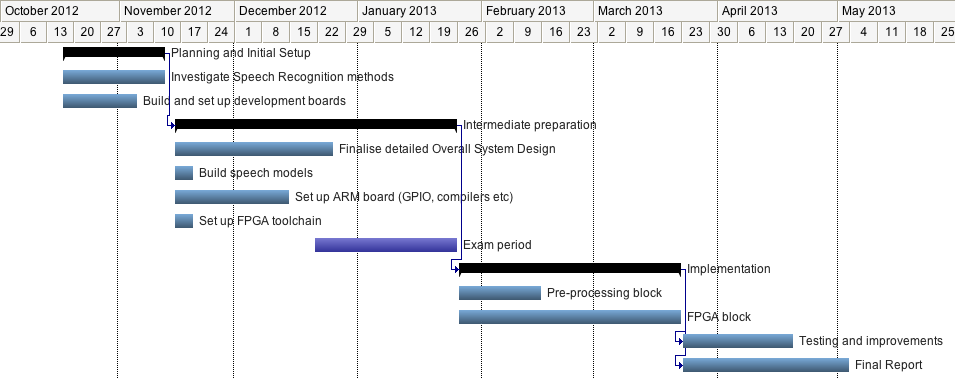
\includegraphics[width=1.4\textwidth,angle=90]{gantt-chart-initial.png}
	\end{center}
	\caption{First Gantt chart with high expectations}
	\label{fig:gantt1}
\end{figure}

\begin{figure}[tb]
	\begin{center}
		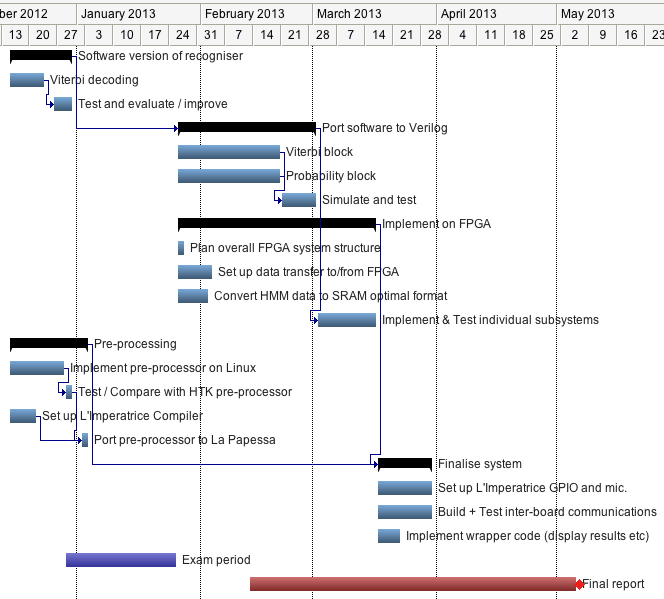
\includegraphics[width=1.1\textwidth,angle=90]{gantt-chart-interim.png}
	\end{center}
	\caption{Interim Gantt chart for remaining work}
	\label{fig:gantt2}
\end{figure}
% section overview (end)


\section{Considerations} % (fold)
\label{sec:details_of_tasks}
In the event that pre-processing code is too hard or time consuming to write, the alternative is to use the HTK to do it, and test the speech recognition offline.  Initialy all development of the system will use the HTK generated MFCC files, as there is certainty that they are correct.  This will allow focus to remain on the more interesting problem of implementing a viterbi decoder block in hardware.

The Voxforge models may be far too complex to use for the project, as straightforward Viterbi decoding is not sufficient for larger models.  If this is the case, there are several options that have been investigated, and neither would take much time.  The HTK is capable of reducing model size by using clustering and regression trees.  Another option would be to train a very simple model from scratch, possibly using the audio and transcriptions available on Voxforge.  However, the priority is to build the system, and if the model is found to be too large it can be adapted.

It may be that the Spartan 3AN FPGA on La Papessa will be too small to hold the system code.  If this is the case, the University has several Altera DE0 evaluation boards that have much more space, with the only downside being that this moves away from the Micro Arcana family.  

% section details_of_tasks (end)


% chapter plan_of_remaining_work (end)

%% ----------------------------------------------------------------
\appendix
%!TEX root = Main.tex
% Appendix A


% Needed in Appendices:
%----------------------
%
% Detailed Doc of development environment for La Papessa and L'Imperatrice
%
% Scripts and info for Voxforge model creation / adaption
\backmatter
\bibliographystyle{plainnat}  % TODO: fix ecs bib style...
\bibliography{../citations-ALL}
\end{document}
%% ----------------------------------------------------------------
